\documentclass[master.tex]{subfiles}
\begin{document}

\chapter{Specification}
\label{chap:specification}

After gaining some familiarity with Phometa in the previous chapters, this
chapter provides a complete reference of Phometa. After reading this chapter,
you should be able to use Phometa in full efficiency.

\section{User Interface Overview}

After you install and start Phometa according to appendix chapter
\ref{chap:installation_startup}, the program will look like this in a web-browser.

\begin{figure}[H]
    \centering
    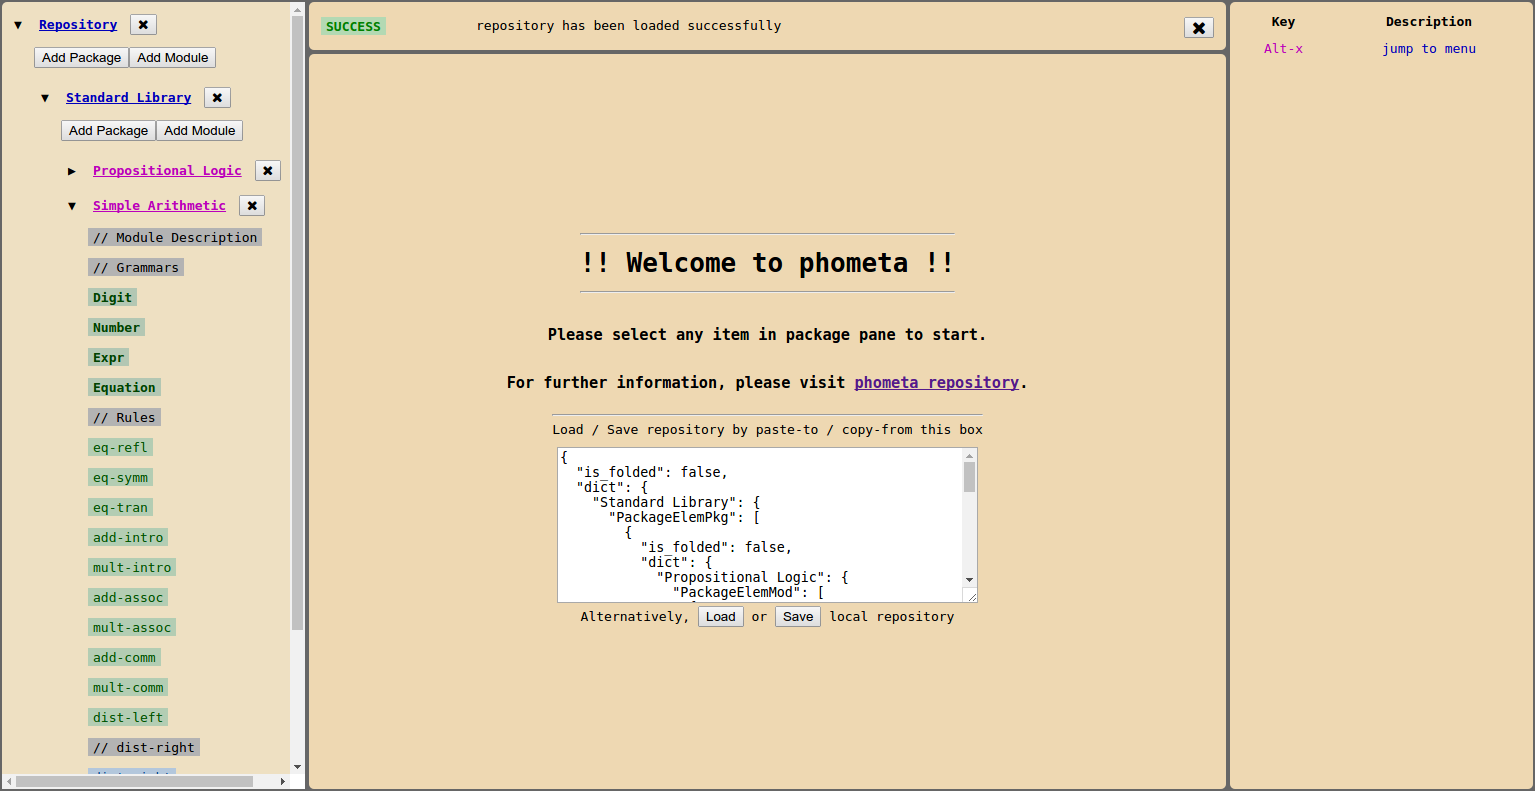
\includegraphics[width=\textwidth]{spec-window-when-start}
    \caption{Screenshot of Phometa when you open it from web-browser.}
\label{fig:specification-phometa-home-window}
\end{figure}

According to figure \ref{fig:specification-phometa-home-window}, user interface
of Phometa is divided into 4 panes as the following

\begin{itemize}
\item\textbf{Package Pane (left)} --- shows and let users interact with the
  global structure of proofs repository.
\item\textbf{Keymap Pane (right)} --- shows every possible key-binding on the
  current state of the program, user can also click any row directly to get the
  same effect as pressing the corresponded key.
\item\textbf{Grids Pane (centre)} --- shows and lets user interact with the
  current content, grids the pane can be split into several sub-panes using mode
  menu explained below.
\item\textbf{Messages Pane (upper-centre)} --- show incoming notifications such
  as success or user exception notification; if there isn't any notification,
  this pane will disappear.
\end{itemize}

On any state of the program, user can click \pkbd{Alt-x} to jump to menu,
this will change the keymap pane to display the following key-bindings

\begin{itemize}
\item \pkbd{l} --- reload proofs repository from \texttt{repository.json}
\item \pkbd{s} --- save proofs repository to \texttt{repository.json}
\item \pkbd{1} --- reform the grids pane to display just 1 sub-pane
\item \pkbd{2} --- reform the grids pane to display 2 sub-panes aligned
  horizontally.
\item \pkbd{3} --- reform the grids pane to display 3 sub-panes aligned
  horizontally.
\item \pkbd{4} --- reform the grids pane to display 4 sub-panes as $2 \times 2$
  grids.
\item \pkbd{8} --- reform the grids pane to display 2 sub-panes aligned
  vertically.
\item \pkbd{9} --- reform the grids pane to display 3 sub-panes aligned
  vertically.
\item \pkbd{h} --- make focused sub-pane of the grids pane display home page
\item \pkbd{p} --- toggle (show / hide) the package pane
\item \pkbd{k} --- toggle (show / hide) the keymap pane
\end{itemize}

For example, in any state of the program, we can split the grids pane into two
horizontally sub-panes by pressing \pkbd{Alt-x} followed by \pkbd{2} to get a
result similar to figure \ref{fig:specification-1x2-grids}.

In fact, splitting grids is recommended when you construct a proof, because it
will let you use one of the sub-panes to look up relevant grammars and rules
without losing concentration on a theorem that is on another sub-pane.

\begin{figure}[H]
    \centering
    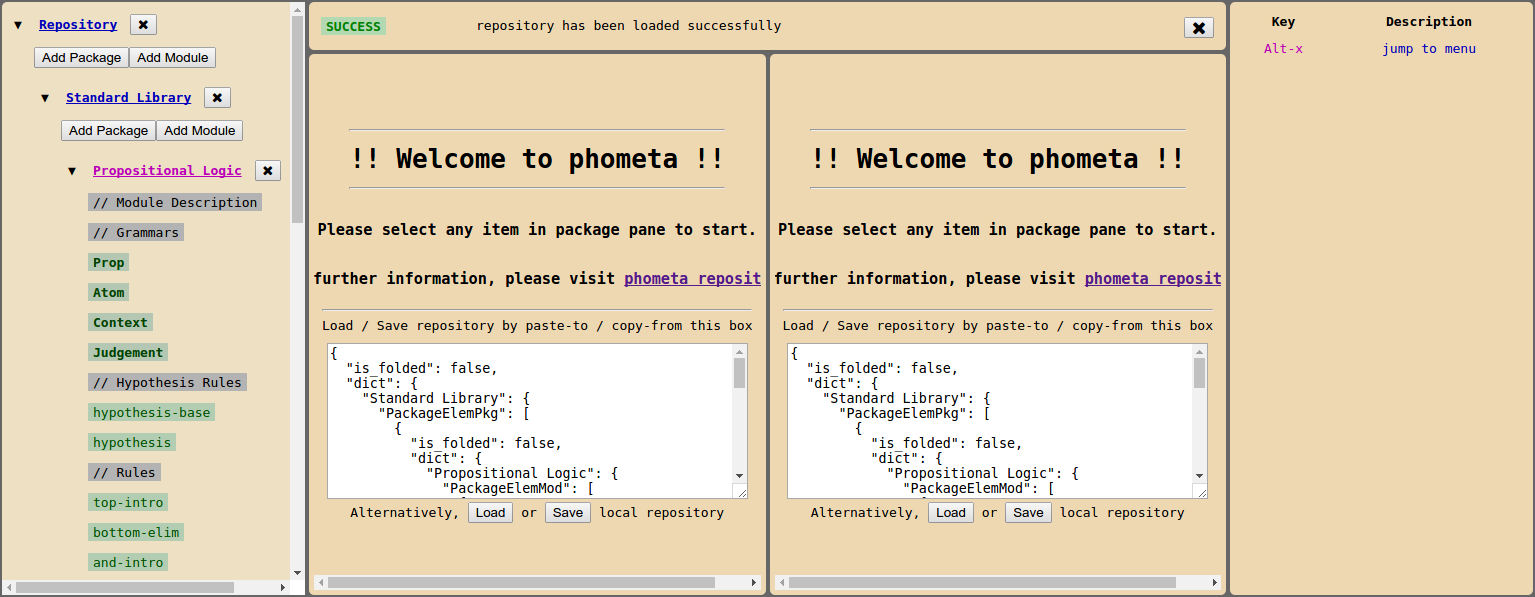
\includegraphics[width=\textwidth]{spec-1x2-grids}
    \caption{Screenshot of Phometa when you split the grids pane into $1 \times 2$
      grids.}
\label{fig:specification-1x2-grids}
\end{figure}

\section{Auto-Complete Input Box}
Although users will interact with Phometa mainly by clicking a button and
pressing a keyboard shortcut, there are several places that might require the
user to type something, and in order make this as convenient as possible, every
input box except textarea in comment node will have \emph{auto-complete}
functionality.

An (auto-complete) input box will internally have a list of choices, which will
be mapped to keys \pkbd{Alt-{1..9}} respectively. Because these choices are
keyboard shortcut hence they will be visible in the keymap pane so user can see all
of this. If there are more than 9 choices, it will map just the first 9 choices to
\pkbd{Alt-\{1..9\}} and provide \pkbd{Alt-[} and \pkbd{Alt-]} that can jump to
previous and next page of choices respectively.

\begin{figure}[H]
    \centering

\begin{minipage}{0.35\textwidth}
\begin{flushleft}
    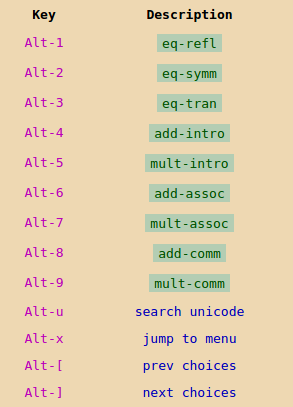
\includegraphics[width=\textwidth]{spec-autocomplete-1}
\end{flushleft}
\end{minipage}
~
\begin{minipage}{0.35\textwidth}
\begin{flushright}
    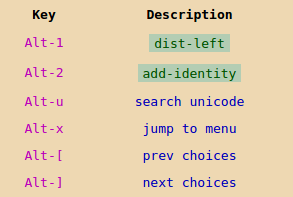
\includegraphics[width=\textwidth]{spec-autocomplete-2}
\end{flushright}
\end{minipage}
\caption{Key-blinding of an example of auto-complete before and after pressing \pkbd{Alt-]}}
\label{fig:specification-autocomplete-choices}
\end{figure}

Another way to access further choices is to type some sub-strings (separated by
space) in the input box. This will filter only choices that still match with
those sub-string. For example, according to the choices in figure
\ref{fig:specification-autocomplete-choices}, if we type \texttt{``dd''}, it
will match just 4 rules which are \prule{add-intro}, \prule{add-assoc},
\prule{add-comm}, \prule{add-identity} since this has \texttt{``dd''} as
sub-string. Now, if we type \texttt{``dd in''} it will match just
\prule{add-intro} since it is the only one that has \texttt{``dd''} \emph{and}
\texttt{``in''} as sub-string. In addition, if there is just one choice left, we
can hit ``Return'' for that choice alternative to \pkbd{Alt-1} for convenience.

\begin{figure}[H]
    \centering

\begin{minipage}{0.35\textwidth}
\begin{flushleft}
    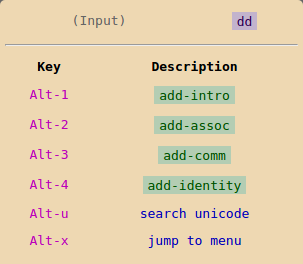
\includegraphics[width=\textwidth]{spec-autocomplete-3}
\end{flushleft}
\end{minipage}
~
\begin{minipage}{0.35\textwidth}
\begin{flushright}
    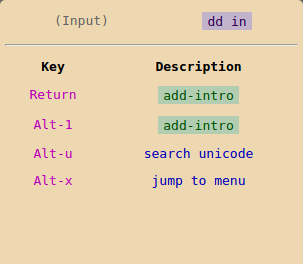
\includegraphics[width=\textwidth]{spec-autocomplete-4}
\end{flushright}
\end{minipage}
\caption{Keymap pane of figure \ref{fig:specification-autocomplete-choices}
  after be filtered by \texttt{``dd''} and \texttt{``dd in''}.}
\label{fig:specification-autocomplete-choices-filtered}
\end{figure}

When typing something into the input box, it also appears on the top of the
keymap pane as well (example as in figure
\ref{fig:specification-autocomplete-choices-filtered}). Although it is not
related to keyboard shortcut but that position is closer to the keymap table,
hence user can type the filter then look at the remaining choices more easily.

Some input box can accept newly created string as well e.g.\ input box waiting
for the name of a new node. If this is the case, you can write the string
directly into the input box then hit \pkbd{Return} to complete it\footnote{If
  you click somewhere else before hitting \pkbd{Return}, the string in the
  input box will be gone without producing any effect. This common pitfall for
  newcomers and will be explain further in chapter
  \ref{chap:evaluation_conclusion}.}. Please note that the written string still
be used to filter choices out (if exists), but \pkbd{Return} as alternative to
\pkbd{Alt-1} will no longer work as it contradicts with this new key.

Auto-complete is also capable for unicode input method as well, if you want to
add a unicode character, just press \pkbd{Alt-u} then the keymap pane will look
like figure \ref{fig:specification-autocomplete-choices-unicode}.

In unicode input method, we have choices that map to each unicode character
using its name in \LaTeX\ math mode, these choices can be manipulated by
\pkbd{Alt-[} and \pkbd{Alt-]} and filtering method similar to normal choices
above. Once a choice is selected, it will be appended to the end in input box
and return to normal input method. However, if you enter unicode input method by
accident you can press \pkbd{Escape} to return to normal input method with
appending any unicode character.

\begin{figure}[H]
    \centering

\begin{minipage}{0.35\textwidth}
\begin{flushleft}
    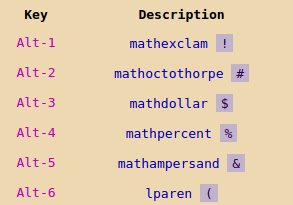
\includegraphics[width=\textwidth]{spec-autocomplete-5}
\end{flushleft}
\end{minipage}
~
\begin{minipage}{0.35\textwidth}
\begin{flushright}
    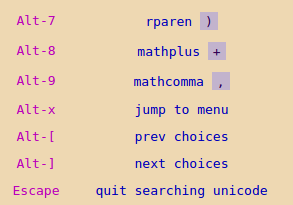
\includegraphics[width=\textwidth]{spec-autocomplete-6}
\end{flushright}
\end{minipage}
\caption{Key-blinding after entering unicode input method.}
\label{fig:specification-autocomplete-choices-unicode}
\end{figure}

To conclude this section, originally, auto-complete was designed for an input
box that is used to select a choice e.g.\ selecting a grammar for a term or
selecting a rule for a step of a theorem, but now it is extended to other types
of input box that doesn't have choice e.g.\ input box the name of a new node. So
all of input boxes will have some feature in common, e.g.\ ability to
use unicode input mode, this reduces Phometa learning curve.

\section{The proofs repository}

Phometa has a repository which consists of packages and modules. Analogously,
you can imagine packages as directories and modules as files, therefore the
proofs repository is similar to a real repository that contains directories and
files.

The package pane represents the global structure as shown in the following
example,

\begin{figure}[H]
    \centering

\begin{minipage}{0.35\textwidth}
\begin{flushleft}
    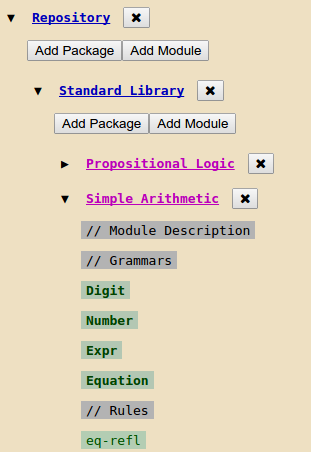
\includegraphics[width=\textwidth]{spec-package-pane-1}
\end{flushleft}
\end{minipage}
~
\begin{minipage}{0.35\textwidth}
\begin{flushright}
    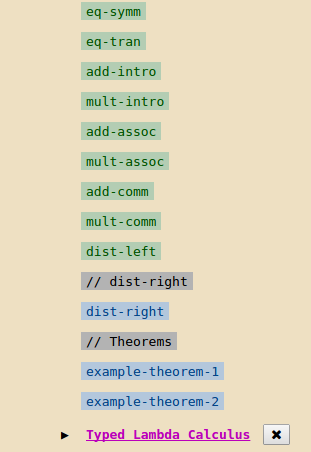
\includegraphics[width=\textwidth]{spec-package-pane-2}
\end{flushright}
\end{minipage}

\caption{Package pane represents the global structure of proofs repository}
\label{fig:specification-package-pane}
\end{figure}

The current repository has one package named ``Standard Library'' which consists
of three modules named ``Propositional Logic'', ``Simple Arithmetic'', and
``Typed Lambda Calculus''. Each module of Phometa consists of a sequence of
nodes, each node can be either comment (grey), grammar (dark green), rule (light
green), or theorem (blue).

Please note that a package contains its elements alphabetically whereas a
modules contains its nodes using an explicit ordering that user can swap among
them later.

Each package and module can be folded or unfolded by clicking a triangle in
front of it. You can also delete them by clicking \closeButton\ on the right
hand side, then the conformation notification will appear in the messages pane
like this


\includegraphics[width=\textwidth]{spec-delete-confirmation.png}

You can add sub-packages or sub-modules in any package by clicking ``Add
Package'' or ``Add Module'' respectively, the clicked button will transform to
an input box that you can enter the name.

To read or edit a module, you can click at the label of the module directly,
this will make the focused sub-pane\footnote{If there isn't a focus one, use the
  first sub-pane.} of the grids pane to display the module similar to figure
\ref{fig:specification-module}.

\begin{figure}[H]
    \centering
    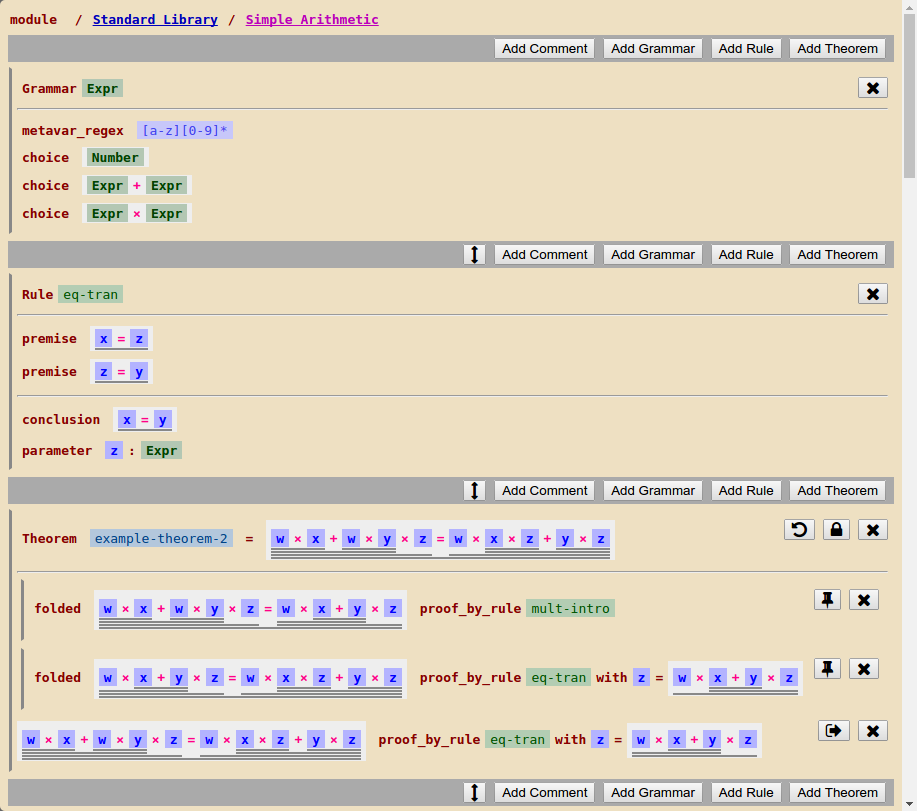
\includegraphics[width=0.7\textwidth]{spec-module}
    \caption{Screenshot of Simple Arithmetic module displayed in the grids pane
      after the user click the label ``Simple Arithmetic'' in the package pane.
      Please note that nodes in this module are reordered so you can see
      different type of nodes in one screenshot.}
    \label{fig:specification-module}
\end{figure}

The displayed module contains nodes that you can interact\footnote{Details on
  how to interact with each type of nodes will be describe in later sections.}
with directly. If you feel like this is too crowded, you can concentrate on
particular node by clicking its label in the package pane, this will show only
that node on the grids pane not the entire module.

Nodes in a module are interspersed by panels which allow you add a new node by
clicking the button corresponded to the type of a new node, the button then
change to an (auto-complete) input box that ask for the name of that node, after
you type the name and hit \pkbd{Return}, the new node will appear at the
position of that panel. A panel also has \swapButton\ that allow you to swap the
location between the above and below nodes.

The current proofs repository can be loaded or saved with
\texttt{repository.json} by using \pkbd{Alt-x l} and \pkbd{Alt-x s} as we
mention before. This allows user to manipulate the proofs repository directly.
For example,
\begin{itemize}
\item User can backup the current state of proofs repository by copy
  \texttt{repository.json} to somewhere else. If user accidentally delete some node
  or something else gone wrong, user can just replace it with the backup one.
\item Users can work in a group on the same repository by passing
  \texttt{repository.json} around.
\item Users can distribute their formal systems to others by publishing their
  \texttt{repository.json}
\end{itemize}
However, manually modifying \texttt{repository.json} without using Phometa
interface is strongly discouraged as it will render the repository into an
inconsistent state.

Alternative to \texttt{repository.json}, user can copy / paste the repository
directly from the text-area in the home page.

\section{Node Comment}

Node comment allows users to add commentary anywhere in a module. It is a proper
node i.e.\ we need to specify the name of the comment, by convention, we will
add ``\textbackslash\textbackslash'' as the prefix to the name so we don't have
to worry about name clash with another type of nodes.

To construct this, we need to obtain a blank node using one of adding panels
explained in the last section. Then you can click ``Edit Comment'' which is on
the top-right corner of the node then a HTML textarea\footnote{This is the only
  input box that doesn't have auto-complete functionality.} will appear so you can
write your comment, once it is finished, you can click ``Quit Editing'' button
(or simply click somewhere else), this will transform the HTML textarea to
normal box. Unlike other nodes, there is no need to lock a comment node so you
can come back and edit this anytime.

\section{Node Grammar}

Node grammar allows users to encode a Backus-Naur Form. To construct this, we
need get a draft grammar using one of adding panels, this will let us define the
following properties of the grammar

\begin{itemize}
\item \kMetaVarRegex\ --- Specify JavaScript regex pattern that control the name
  of a meta variable of this grammar. This property is optional, and if it is
  absent, meta variables of this grammar cannot be instantiated.
\item \kLiteralRegex\ --- Specify JavaScript regex pattern that control the name
  of a literal of this grammar. This property is optional, and if it is
  absent, literal of this grammar cannot be instantiated.
\item \kChoice\ --- Describe an alternative branch that a term can be
  instantiated to. A choice consists of sub-grammars and format-strings stripped
  to each other.

  This property is multiple, you can create a new choice by clicking ``Add
  Choice'' button on the top-right corner of the grammar, it will ask you for
  the number of sub-grammars that the new choice will have, after that, a new
  \kChoice\ will appear with $2n + 1$ buttons, the odd buttons will asking for
  string of syntax, and even buttons will be asking for sub-grammar (draft
  grammar and itself included) which you can use auto-complete method described
  in auto-complete section to complete.

  You can also swap order among choices by clicking \swapButton\ on the right
  hand side of that choice, this will swap the current choice with the one lower
  (wrap around if necessary).
\end{itemize}

\begin{figure}[H]
    \centering

\begin{minipage}{0.48\textwidth}
\begin{flushleft}
    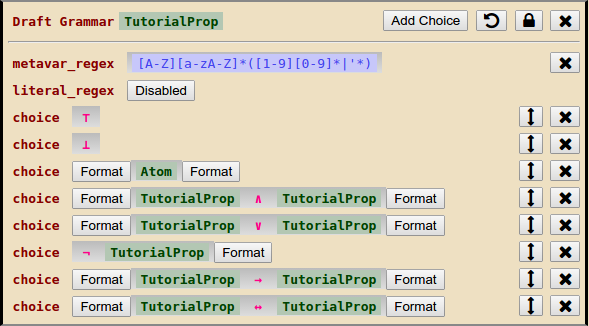
\includegraphics[width=\textwidth]{prop-tut-prop-5}
\end{flushleft}
\end{minipage}
~
\begin{minipage}{0.48\textwidth}
\begin{flushright}
    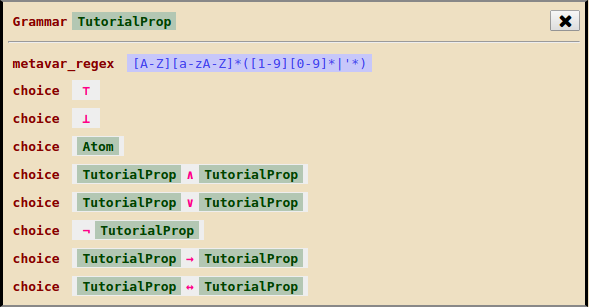
\includegraphics[width=\textwidth]{prop-tut-prop-6}
\end{flushright}
\end{minipage}
\caption{Example of a grammar before and after it is locked.}
\end{figure}

Once the grammar is completed i.e.\ all of buttons asking for sub-grammars are
fulfilled, we can lock it using \lockButton\ on the top-right corner of the
grammar so it will become a proper grammar and ready for usage of other type of
nodes. In addition, if something is wrong during constructing this, you can
reset the grammar to the initial state by clicking \resetButton.

For more information about grammar construction, see appendix section
\ref{sec:how_to_built_grammars_and_rules}.

\section{Root Term}

Root terms are not sub-terms of any other terms (as you can see from user
interface). There 3 types of terms depending in its editability as the following
\begin{itemize}
\item Editable-up-to-grammar --- Both of grammar and term content of a root term
  can be changed. They are used to construct premises and the conclusion of
  rules and the goal of theorems.
\item Editable-up-to-term --- Term content of a root term it editable
 but the grammar is given and fixed. It is used in the place that depend on
 other node such as an argument of a rule.
\item Read-only --- Everything is fixed, the root term is shown there only for
  your information.
\end{itemize}

To make this type more distinguishable, read-only root-term will have white
background colour represented its immutability, in constant, other two will have
grey background colour.

When an editable-up-to-grammar root-term is newly created, it doesn't know its
own grammar and it will be shown as a button with a label ``Choose Grammar''. To
specify a grammar, click that button, it will transform to an auto-complete
input box waiting you to select a grammar using the method described in
auto-complete section. Once you select a grammar for this, it will transform to
another auto-complete input box but now asking for term content which behaves
the same as an editable-up-to-term root-term.

At the beginning of term-content input-method, i.e.\ when editable-up-to-grammar
root-term get its grammar or editable-up-to-term root-term is newly created, the
root term will show a single auto-complete input box with a placeholder as the
name of corresponding grammar and have green background colour. This
auto-complete input box, from now on, will be called \emph{todo-hole} and it can
be fulfilled one of following method

\begin{itemize}
\item Select one of \kChoice{}s stated in the corresponding grammar declaration
  using auto-complete method,
  this will replace current todo-hole with that choice with corresponding
  sub-grammars as further todo-holes (if any).
\item Write a string to the input box and hit \pkbd{Return}
  \begin{itemize}
  \item if the string match with \kMetaVarRegex, then the current todo-holes
    will be replaced with meta variable
  \item otherwise, if the string match with \kLiteralRegex, then the current
    todo-holes will be replaced with literal
  \item otherwise, do nothing and prompt an exception on the messages pane.
  \end{itemize}
\item Select on of existing meta variables or literals (if any) using
  auto-complete method.
\end{itemize}

\begin{figure}[H]
    \centering

\begin{minipage}{0.50\textwidth}
\begin{flushleft}
    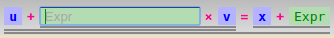
\includegraphics[width=\textwidth]{spec-root-term-1}
\end{flushleft}
\end{minipage}
~
\begin{minipage}{0.35\textwidth}
\begin{flushright}
    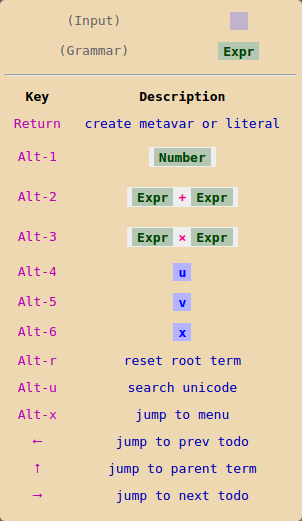
\includegraphics[width=\textwidth]{spec-root-term-2}
\end{flushright}
\end{minipage}
\caption{Example of root term during term-content input-method (left) and the
  corresponding key-blinding (right). You can see that the current todo-hole has
  \pgmr{Expr} as its grammar so their are 3 choices from \pgmr{Expr} and other 3
  choices which are existing meta variables that has been entered bofore,
  nevertheless it can write a new string then hit \pkbd{Return} for meta
  variable as well.}
\label{spec-root-term-todo}
\end{figure}

After the current todo-hole as been fulfilled, the cursor will automatically
focus on the todo-hole, so user can finish entering the whole term content
without touching a mouse.

Phometa also has another feature to automatically expand the term that has
exactly one choice and can't instantiate neither of meta variable nor literal
e.g.\ a term of \pgmr{Equation}

Every (sub) term can be focused directly by clicking at it, then the focused
term will be overlined. If the focused term is todo-hole, keymap show its input
text and grammar (similar to the right screenshot in figure
\ref{spec-root-term-todo}), otherwise, the keymap will show its grammar and the
term (similar to the right screenshot in figure). In addition, if the focus term
is \kChoice\ term, we can jump to its sub-terms using \pkbd{\{0..9\}} as showned
in figure \ref{spec-root-term-non-todo}.

\begin{figure}[H]
    \centering

\begin{minipage}{0.40\textwidth}
\begin{flushleft}
    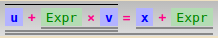
\includegraphics[width=\textwidth]{spec-root-term-3}
\end{flushleft}
\end{minipage}
~
\begin{minipage}{0.35\textwidth}
\begin{flushright}
    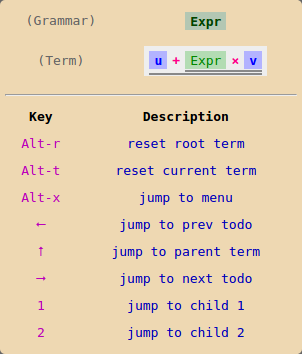
\includegraphics[width=\textwidth]{spec-root-term-4}
\end{flushright}
\end{minipage}
\caption{Example of root term when \kChoice\ term is clicked, we can jump to its
  first term by clicking \pkbd{1} or second term by clicking \pkbd{2}.}
\label{spec-root-term-non-todo}
\end{figure}

Root term has limited space to interact, therefore, it make use lots of shortcut
which can be described\footnote{This list excludes keyboard shortcut of
  auto-complete as it is not specific to root term} as the following

\begin{itemize}
\item \pkbd{r} --- reset the whole root term to its initial state (mutable term only).
\item \pkbd{t} --- reset the current term to todo-hole (mutable and non
  todo-hole term only).
\item \pkbd{Up} --- if it is root term, quit root term and focus on outer nod
\item \pkbd{Up} --- if it is sub term, jump to parent term of current term.
\item \pkbd{Left} --- jump to next todo-hole.
\item \pkbd{Right} --- jump to next todo-hole.
\end{itemize}

For further information about building a root term, please see the first half of
section \ref{sec:arith-theorems-lemmas}.

\section{Node Rule}

Node rule allows users to encode a derivation rule. To construct this, we need
get a draft rule using one of adding panels, this will let us define the
following properties of the rule

\begin{itemize}
\item \kAllowReduction\ --- Specify whether this rule could be used for meta
  reduction or not. This property is a flag i.e.\ you can click
  ``Disabled''/``Enabled'' button to toggle it.
\item \kConclusion\ --- Specify a root term that will be used as the conclusion
  of the rule. The root term displayed here is editable-up-to-grammar where you
  can fulfil it using method described in the last section.
\item \kPremise\ --- Describe a root term that will be used as one of premises
  of this rule. Root term input method is the same as \kConclusion{}.

  This property is multiple, you can create a new precise by clicking ``Add
  Premise'' button on the top-right corner of the rule.
\item \kCascade\ --- Describe a cascade premise which similar to a normal
  premise but when the rule is called, rather than doing normal pattern
  substitution, it tries to call its first sub-rule, if success this cascade
  premise will be replaced by zero-or-more premises of sub-rule, otherwise,
  cascadely calling other sub-rules. For more information about a cascade
  premise, please see appendix section \ref{sec:hypothesis_rules}.

  This property is multiple, you can create a new cascade premise by clicking
  ``Add Cascade'' button on the top-right corner of the rule.

  Each cascade premise has a list of sub-rules that it can try cascade. To add a
  new sub-rule click ``Add Sub-Rule'' button which will transform to an
  auto-complete input box asking for a rule (draft rules and itself included),
  then the sub-rule calling template consists of the following
  \begin{itemize}
  \item Sub-rule name --- The rule that will be called as sub-rule, this is
    specified when we add this sub-rule calling template and now it is fixed.
  \item Unifiable / Exact Match flag --- The flag that you can
    toggle between ``Unifiable''  (which is the default)  and ``Exact Match''
    (treat sub-rule that require further substitution as failure).
  \item Pattern of sub-rule goal --- An editable-up-to-term root-term that is
    formed to match against sub-rule conclusion.
  \item Patterns of sub-rule arguments --- Editable-up-to-term root-terms that
    are formed to match against sub-rule parameters.
  \end{itemize}
  You can use \swapButton\ to reordering sub-rules around in the same way that
  you swap ordering of \kChoice{}s of a grammar.

\item \kParameter{}s --- Show meta variables (literals excluded) that appear
  in one of premises but not in the conclusion. This property is automatic i.e.
  it will be updated every time when one of premises or conclusion is updated,
  user cannot manually change it.
\end{itemize}

List of \kPremise{}s and list of \kCascade{}s are, in fact, the same list, you
can use \swapButton\ to swap ordering of these \kPremise{}s and \kCascade{}s
around in the same way that you swap ordering of \kChoice{}s of a grammar.

\begin{figure}[H]
    \centering

\begin{minipage}{0.48\textwidth}
\begin{flushleft}
    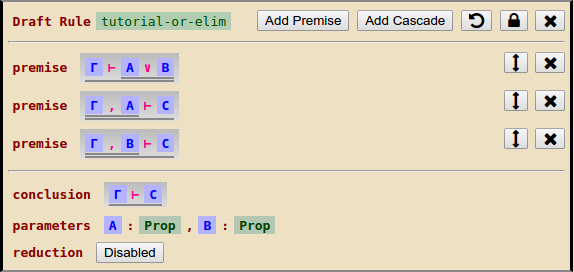
\includegraphics[width=\textwidth]{prop-tut-or-elim-5}
    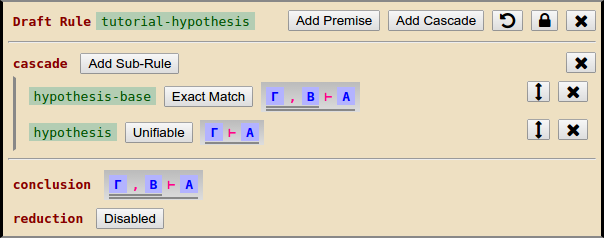
\includegraphics[width=\textwidth]{prop-tut-rule-hypo-5}
\end{flushleft}
\end{minipage}
~
\begin{minipage}{0.48\textwidth}
\begin{flushright}
    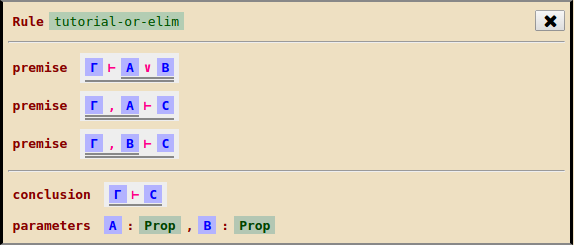
\includegraphics[width=\textwidth]{prop-tut-or-elim-6}
    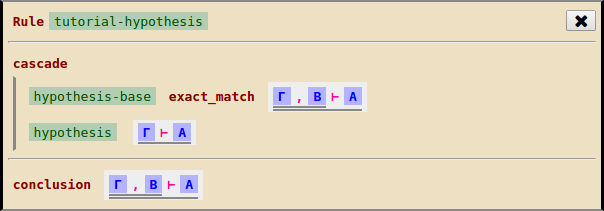
\includegraphics[width=\textwidth]{prop-tut-rule-hypo-6}
\end{flushright}
\end{minipage}
\caption{Example of rules before and after they are locked.}
\end{figure}

Once the rule is completed i.e.\ all of root terms has no todo-hole left, we can
lock it using \lockButton\ on the top-right corner of the rule so it will
become a proper rule and ready for usage of other type of nodes. In addition,
if something is wrong during constructing this, you can reset the rule to the
initial state by clicking \resetButton.

For more information about rule construction, see appendix section
\ref{sec:how_to_built_grammars_and_rules}.

\section{Node Theorem}

\subsection{Theorem Construction}

Node theorem allows users to encode a derivation tree. To construct this, we
need get a draft theorem using one of adding panels, this will give us a blank
theorem with the goal as editable-up-to-grammar root-term.

\begin{center}
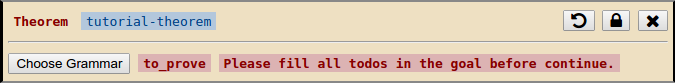
\includegraphics[width=0.8\textwidth]{spec-thm-1}
\end{center}

Once the we complete the goal, it will also appear in the header\footnote{This
  is useful for a long theorem as reader doesn't need to scroll down the very
  end just to see what has been proven.} and there might be two buttons pop-up
as the following

\begin{center}
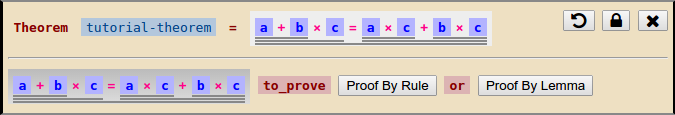
\includegraphics[width=0.8\textwidth]{spec-thm-2}
\end{center}

\begin{itemize}
\item ``Proof By Rule'' button --- once clicked, it will turn to an
  auto-complete input box with choices consisting of rules which has the grammar
  of the conclusion the same as the grammar of the current goal. If there is no
  such a rule, ``Proof By Rule'' button will not appear at the first place.
  Please note that some rule on auto-complete choices might not be applicable to
  the current goal, if we select it, it will nothing and pop-up exception in the
  message pane.
\item ``Proof By Lemma'' button --- once clicked, it will turn to an
  auto-complete input box with choices consisting of lemmas which each of them
  has the goal that can turn to out current goal i.e.\ each meta variable of the
  lemma goal can be substituted in such a way that is it identical to out
  current goal. If there is no such a lemma, ``Proof By Rule'' button will not
  appear at the first place. In fact, if there is at least one lemma in the
  auto-complete choices, we can guarantee that our current goal can be proven as
  it can fail in the similar way as rules.
\end{itemize}

In the current example, we could ``Proof By Lemma'' and select \pthm{dist-left}
then this theorem will finish immediately, but in order to investigate more on
other thing, we will select ``Proof By Lemma'' and select \prule{eq-tran}.

Normally, when we apply a rule, the conclusion of the rule will be pattern
matched against the current goal, then substitute pattern match result to each
premise to get sub-goals that are needed to be proven later. However if the rule
has parameters, it will ask user to fill arguments that corresponding to each
parameter using an editable-up-to-term root-term, similar to this example.

\begin{center}
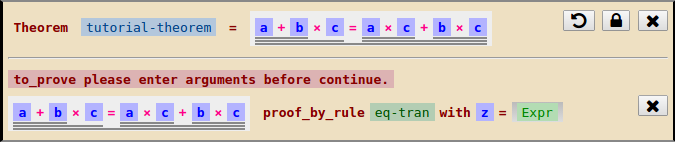
\includegraphics[width=0.8\textwidth]{spec-thm-3}
\end{center}
\begin{center}
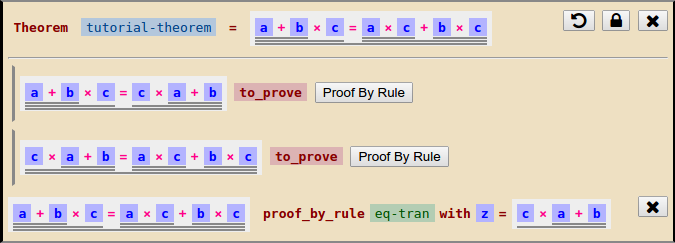
\includegraphics[width=0.8\textwidth]{spec-thm-4}
\end{center}

After the main goal knows its rule or lemma, the colour of it become white i.e.
now it is read-only root-term. Sub-goals (if any) will have white background as
well since they depend on a rule and it can't be changed.

The generated sub-goals can be proven using the same method as the main goal,
and it will happened recursively until all leaf sub-goals are proven by rules
with no premises or by lemma.

For each (sub) goal, that has been proven, we can reset its proof by clicking
\closeButton\ on the bottom-right corner of particular proof. If we reset the
main proof, the theorem goal will turn grey again and allow we to modify it.

Once, the theorem is complete i.e.\ there is no active sub-goal left, we can
lock a theorem to become a lemma by clicking \lockButton\ on the top-right
corner of the theorem. In addition, if something is wrong during constructing
this, you can reset the entire theorem to the initial state by clicking
\resetButton.

Since user will interact with Phometa most the time by constructing a theorem,
so we provide some keyboard short-cut that user can use.

\begin{itemize}
\item \pkbd{r} --- reset the whole theorem (equivalent to \resetButton).
\item \pkbd{t} --- reset the current current proof (equivalent to \closeButton\
  of the current proof).
\item \pkbd{l} --- lock the theorem (equivalent to \lockButton).
\end{itemize}

For further information about building a theorem, please see the second half of
section \ref{sec:arith-theorems-lemmas}.

\subsection{Theorem Fold/Unfold}

Some (sub) proof in a theorem is quite long so its goal and sub-goals will be
far away from each other, therefore, it is very hard to read them together as an
instance of a derivation rule. To tackle this problem, we can click
\focusButton\ on the proof that we want to focus, this will fold its sub-proofs
so goal and sub-goals will stick together and easier to read as instance of a
derivation rule.

To unfocus the proof, we can click \unfocusButton\ at the same position that we
click \focusButton. This will unfold all of sub-proofs that are currently
folded.

To avoid potential confusions among (sub) proofs, we allow to have a focus proof
one at the time (per theorem) i.e.\ if you click \focusButton\ on some proof
during another proof is being focus, then it will automatically unfocus the old
one (without clicking \unfocusButton) and then focus the new one.

Some proof might not have any sub-goal that is foldable, focusing on it will not
produce any difference, hence, such a proof will simply doesn't have
\focusButton\ at the first place.

For further information about theorem fold/unfold, please see section
\ref{sec:arith-complex-theorem}.

\section{Meta Reduction}

Some rule has exactly one premise which has the same grammar as the conclusion.
Conceptually, this establishes some kind of relation that suggests that the
conclusion of this rule should be able to \emph{reduce} to the premise. We can
make this concept come true by enabling flag \kAllowReduction\ on that rule.

Meta reduction can be performed in a (sub)term that is inside a (sub)goal of a
theorem, and that (sub)goal must be in ``todo'' state i.e.\ it must not be in
parameters-waiting state nor has been proven by a rule or a lemma. Although
sub-goal is read-only root-term but meta reduction can be preform since it is
not related to the term construction.

Once you click such a (sub)term, you might see some rule appear as an
auto-complete choice, this means that you can use that rule to reduce the term.

Formally, a rule can appear as an auto-complete choice to reduce a term if it
satisfies the following condition
\begin{itemize}
\item The \kAllowReduction flag of the rule is set.
\item The rule requires no parameters.
\item The generates exactly one premise (might happen dynamically via cascade
  premises).
\item That premise has the same grammar as the conclusion of the rule.
\item The applying process doesn't involve any further substitution.
\end{itemize}

For further information about meta-reduction, please see appendix section
\ref{sec:prop-context-manipulation}.

\end{document}
